%% LyX 2.1.1 created this file.  For more info, see http://www.lyx.org/.
%% Do not edit unless you really know what you are doing.
\documentclass[english,a4paper]{article}
\usepackage[T1]{fontenc}
\usepackage{babel}
\usepackage{multicol}
\usepackage{xtab}
\usepackage{graphicx}

\usepackage{geometry}
\geometry{verbose,tmargin=2cm,bmargin=2cm,lmargin=2cm,rmargin=2cm}


\usepackage{minted}
\newminted{python}{mathescape,linenos,numbersep=5pt,autogobble=true,frame=lines,framesep=2mm}
\newminted{pycon}{mathescape,linenos,numbersep=5pt,autogobble=true,frame=lines,framesep=2mm}
\newminted{shell-session}{mathescape,linenos,numbersep=5pt,autogobble=true,frame=lines,framesep=2mm}
\newmintedfile[pythoncodefile]{python}{
%bgcolor=mintedbackground,
fontfamily=tt,
linenos=true,
numberblanklines=true,
numbersep=12pt,
numbersep=5pt,
gobble=0,
frame=leftline,
framerule=0.4pt,
framesep=2mm,
funcnamehighlighting=true,
tabsize=4,
obeytabs=false,
mathescape=false
samepage=false, %with this setting you can force the list to appear on the same page
showspaces=false,
showtabs =false,
texcl=false,
}

\setlength{\parskip}{0.5em plus4mm minus3mm}
\title{QuBricks Documentation}

\begin{document}


  \vspace*{\fill}


  
\includegraphics[width=\textwidth]{qubricks_logo}
  \textcolor{red}{This documentation is a work in progress. If you are interested in using QuBricks, please get in touch with me at
  	mister.wardrop@gmail.com; which will greatly enhance my motivation toward completing this documentation. If you need QuBricks
  	to be extended for your work, I am more than willing to be involved.}

  \vspace*{\fill}
  \vspace*{\fill}



\newpage

  \maketitle

QuBricks is a toolkit for the analysis and simulation of quantum systems in Python.
The primary goal of QuBricks
is to facilitate insight into quantum systems; rather than to be the fastest or most
efficient simulator. As such, the design of QuBricks is not especially geared toward
very large or complicated quantum systems.
It distinguishes itself from toolkits like QuTip\ref{qutip} in that before simulations,
everything can be expressed symbolically; allowing for analytic observations
and computations. Simulations are nonetheless performed numerically, with various
optimisations performed to make them more efficient.

Basic operations are unit-tested with reference to a simple two-level system.


\section{Installation}

QuBricks depends upon {\tt python-parameters} >= 1.1.9, which is available from
GitHub or pypi. Once python-parameters is installed, installing the QuBricks module is
done in one line:
\begin{shell-sessioncode}
  $ python2 setup.py install
\end{shell-sessioncode}

If you run Arch Linux, you can instead install {\tt python-qubricks}
via your package manager using:
\begin{shell-sessioncode}
  $ makepkg -i
\end{shell-sessioncode}


\section{Usage Overview}

The main purpose of this documentation is to demonstrate how to use QuBricks, rather
than to explain the mechanisms of how it works; though there is obviously some overlap.
In section \ref{sec:basic_usage} we demonstrate some extremely basic use cases, before
exploring more interesting cases in section \ref{sec:advanced_usage}.

In the following, we assume that the following has been run:
\begin{pyconcode}
  >>> from qubricks import Operator, QuantumSystem...
  >>> import numpy as np
\end{pyconcode}

\subsection{Basic Usage\label{sec:basic_usage}}
In this section, we motivate the use of QuBricks in simple quantum systems. We will
make use of the submodule {\tt qubricks.wall}, which brings together many of the ``bricks''
that make up QuBricks into usable standalone tools.

Consider a single isolated electron in a magnetic field aligned with Z axis, and a
noisy magnetic field along the X axis. The Hamiltonian describing the mechanics is:
\begin{eqnarray*}
H & = & \mu_B \left(\begin{array}{cc}
B_z & B_x\\
B_x & -B_z
\end{array}\right),
\end{eqnarray*} where $B_z$ is the magnetic field along $z$ and $B_x= B_{x0} + \tilde{B_x}$ is a noise field along $x$ centred
on some nominal value $B_{x0}$ with a high frequency noise component $\tilde{B_x}$. We assume the noise is white:
\[ \left< (B_x-B_{x0})_{t} (B_x-B_{x0})_{t^\prime} \right> = D\delta(t-t^\prime), \] and model it using a
Lindblad superoperator.

This is a simple system which can be analytically solved easily in the absence of noise.
Evolution under this Hamiltonian will lead to the electron's spin gyrating around an axis between
Z and X (i.e. at an angle $\theta = \tan^{-1}(B_z/J_x)$ from the x-axis) at a frequency of $2\sqrt{B_z^2 + B_x^2}$.
The effect of high frequency noise in $B_x$ will continually increase the mixedness in the Z quadrature
until such time as measurements of Z are unbiased. The effect of noise can also be reasonably
simply computed, at least to first order. For example, when $B_z=0$, the return probability for an initially up state
is given by: $p = \frac{1}{2}(1+\cos{2B_{x}t})$. Given that we know that: $\left< \tilde{B_{x}}^2 \right>_{\textrm{avg}} = D/t$,
by taylor expanding we find: $\left<p\right> = 1 - Dt$. A more careful analysis finds that:
\[ \left<p\right> = \frac{1}{2}(1+exp(-2Dt)) . \]
It is possible to find approximations for a general $\theta$, but we leave that as an exercise.

The dynamics of the system can be simulated using the code below, where we have chosen $B_z = B_x$,
and so dynamics should evolve as shown in figure \ref{fig:twolevel}.
\begin{figure}
  \centering
  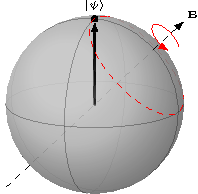
\includegraphics[width=0.4\textwidth]{twolevel.pdf}
  \caption{Dynamics of a single electron spin under a magnetic field aligned 45 degrees
  in the XZ plane.}
  \label{fig:twolevel}
\end{figure}
\pythoncodefile{sqs.py}
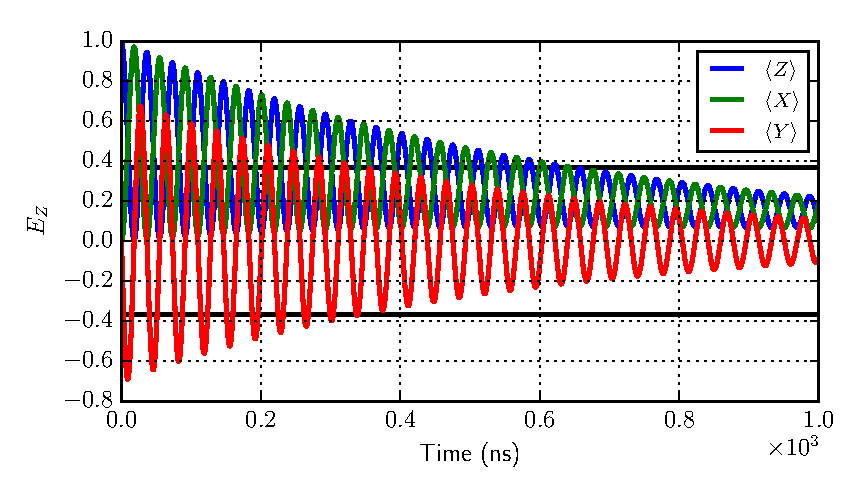
\includegraphics[width=\columnwidth]{results}


\subsection{Advanced Usage\label{sec:advanced_usage}}

For more fine-grained control, one can subclass {\tt QuantumSystem}, {\tt Measurement} and {\tt StateOperator} as necessary. For more information about which
methods are available on these objects, please use the inline python help: help(python-obj).
The templates are as follows:

\pythoncodefile{templates/quantum_system.py}
\pythoncodefile{templates/measurement.py}
\pythoncodefile{templates/state_operator.py}
\pythoncodefile{templates/basis.py}



\section{QuBricks Internals}


\subsection{Operator}
Perhaps the most important brick is the {\tt Operator} object. It represents
all of the two-dimensional linear operators used in QuBricks. The {\tt Operator} object is neither
directly a symbolic or numeric representation of an operator; but can be used to generate
both.

Consider a simple example:
\begin{pyconcode}
  >>> op = Operator(np.array([[1,2],[3,4]]))
  >>> op
  <Operator with shape (2,2)>
\end{pyconcode}

To generate a matrix representation of this object for inspection, we have two
options depending upon whether we want a symbolic or numeric representation.
\begin{pyconcode}
  >>> op() # Numeric representation as a NumPy array
  array([[ 1.+0.j,  2.+0.j],
         [ 3.+0.j,  4.+0.j]])
  >>> op.symbolic() # Symbolic representation as a SymPy matrix
  Matrix([
  [1, 2],
  [3, 4]])
\end{pyconcode}
In this case, there is not much difference.

Creating an {\tt Operator} object with named parameters can be done in two ways.
Either you must create a dictionary relating parameter names to matrix forms, or
you can create a SymPy symbolic matrix. In both cases, one then passes this to
the {\tt Operator} constructor instead of the numpy array above. For example:
\begin{pyconcode}
  >>> op = Operator({'B':[[1,0],[0,-1]], 'J':[[0,1],[1,0]]})
  >>> op.symbolic()
  Matrix([
  [B,  J],
  [J, -B]])
  >>> op.symbolic(J=10)
  Matrix([
  [ B, 10],
  [10, -B]])
  >>> op()
  ValueError: Operator requires use of Parameters object; but none specified.
\end{pyconcode}
When representing {\tt Operator} objects symbolically, we can override some parameters
and perform parameter substitution. We see that attempting to generate a numeric representation of the {\tt Operator}
object failed, because it did not know how to assign a value to $B$ and $J$. Normally,
{\tt Operator} objects will have a reference to a {\tt Parameters} instance (from {\tt python-parameters})
passed to it in the constructor phase, for which these parameters can be extracted. This will in most cases be handled for you by
{\tt QuantumSystem} (see section \ref{sec:QuantumSystem}), but for completeness
there are two keyword arguments you can pass to {\tt Operator} instances: {\tt parameters}, which
shold be a reference to an existing {\tt Parameters} instance, and {\tt basis}, which should
be a reference to an existing {\tt Basis} object or {\tt None} (see \ref{sec:Basis}).
For now, let us manually add it for demonstration purposes.
\begin{pyconcode}
  >>> from parameters import Parameters
  >>> p = Parameters()
  >>> p(B=2,J=1)
  < Parameters with 2 definitions >
  >>> op = Operator({'B':[[1,0],[0,-1]], 'J':[[0,1],[1,0]]},parameters=p)
  >>> op()
  array([[ 2.+0.j,  1.+0.j],
         [ 1.+0.j, -2.+0.j]])
  >>> op(J=10,B=1)
  array([[  1.+0.j,  10.+0.j],
         [ 10.+0.j,  -1.+0.j]])
\end{pyconcode}
We see in the above that we can take advantage of temporary parameter overrides for
numeric representations too [note that a parameters instance is still necessary
for this].

In conjunction with functional dependence inherited from {\tt python-parameters}
this allows for time and/or context dependent operators.

{\tt Operator} objects support basic arithmetic: addition, subtraction, and multiplication using
the standard python syntax. The inverse operation can be performed using the {\tt inverse} method:
\begin{pyconcode}
  >>> op.inverse()
\end{pyconcode}
There is a subclass of the {\tt Operator} class, {\tt OrthogonalOperator}, which
is for operators that have orthogonal eigenvectors; in which case the {\tt inverse}
operation can be greatly simplified.

The Kronecker tensor product can be applied using the {\tt tensor} method:
\begin{pyconcode}
  >>> op.tensor(other_op)
\end{pyconcode}

To apply an {\tt Operator} object to a vector, you can either use the standard
inbuilt multiplication operations, or use the slightly more optimised {\tt apply}
method.

If you are only interested in how a certain variables affect the operator, then
to improve performance you can ``collapse'' the {\tt Operator} down to only
include variables which depend upon those variables.
\begin{pyconcode}
  >>> op.collapse('t',J=1)
\end{pyconcode}
The result of the above command would substitute all variables (with a parameter
override for $J$) that do not depend upon $t$ with their numerical value, and then
perform various optimisations to make further substitutions more efficient. This
is used, for example, in the integrator.

The last set of key methods of the {\tt Operator} object are the {\tt connected}
and {\tt restrict} methods. {\tt Operator.connected} will return the set of all
indicies (of the basis vectors in which the Operator is represented) that are connected
by non-zero matrix elements, subject to the provided parameter substitution. Note that
this comparison is done with the numerical values of the parameters.
\begin{pyconcode}
  >>> op = Operator({'B':[[1,0],[0,-1]], 'J':[[0,1],[1,0]]},parameters=p)
  >>> op.connected(0)
  {0,1}
  >>> op.connected(0,J=0)
  {0}
\end{pyconcode}
The {\tt restrict} method returns a new {\tt Operator} object which keeps only
the entries in the old {\tt Operator} object which correspond to the basis elements
indicated by the indicies.
\begin{pyconcode}
  >>> op = Operator({'B':[[1,0],[0,-1]], 'J':[[0,1],[1,0]]},parameters=p)
  >>> op.restrict(0)
  <Operator with shape (1, 1)>
  >>> op.symbolic()
  Matrix([[B]])
\end{pyconcode}


\end{document}
